% This is LLNCS.DEM the demonstration file of
% the LaTeX macro package from Springer-Verlag
% for Lecture Notes in Computer Science,
% version 2.3 for LaTeX2e
%
\documentclass{llncs}
%
\usepackage{makeidx} % allows for indexgeneration
\usepackage{graphicx}
\usepackage{multicol}
\usepackage{subfigure}
\usepackage{mathptmx} % use Times fonts if available on your TeX system
\usepackage{setspace}
%
\begin{document}
\title{Robotic Validation of an Inter-disciplinary Generic\\
Model of Self-regulated Division of Labour\\ in Social Systems
%\thanks{This research has been funded by the Engineering and Physical Sciences Research Council (EPSRC), UK, grant reference EP/E061915/1.}
}
%\subtitle{Do you have a subtitle?\\ If so, write it here}
\titlerunning{Robotic Validation of an Inter-disciplinary Generic Model\\
of Self-regulated Division of Labour in Social Systems } % if too long for running head
\author{Md Omar Faruque Sarker \and
Torbj{\o}rn S. Dahl %etc.
}
%\authorrunning{Short form of author list} % if too long for running head
\institute{
Robotic Intelligence Lab, University of Wales, Newport, UK\\
\email{Mdomarfaruque.Sarker|Torbjorn.Dahl@newport.ac.uk}
}
%\date{Received: / / Accepted: / / }
% The correct dates will be entered by the editor
\maketitle
\begin{abstract}
Division of labour (DoL) in multi-robot systems or multi-robot task allocation (MRTA) is a challenging research issue in the field of multi-agent and multi-robot systems.
We propose to solve MRTA problems using a set of previously published generic rules for DoL derived from the observation of ant, human and robotic social systems.
These bottom-up rules describe the phenomenon of self-regulated DoL in terms of attractive fields between robots and tasks.
The concrete form of these rules, the \textit{attractive filed model} (AFM), avoids the strong dependence on local interactions found in many existing approaches to MRTA.
We present experimental results that constitute a first validation of AFM as a mechanism for MRTA and as a multi-disciplinary model of self-organisation in social systems.
Our experiments used 16 e-puck robots in a 2m x 2m area.
%\keywords{First keyword \and Second keyword \and More}
%% \PACS{PACS code1 \and PACS code2 \and more}
%% \subclass{MSC code1 \and MSC code2 \and more}
\end{abstract}
%\addtolength{\parskip}{-3.5mm}
\section{Introduction}
\label{sec:intro}
%\vspace{2mm}
Scientific studies show that a large number of animal as well as human social systems grow, evolve and generally continue functioning well by the virtue of their individual self-regulatory mechanism of division of labour (DoL)  \cite{Bonabeau+1999}.
This has been accomplished without any central authority or any explicit planning and coordinating element.
Indirect communication such as stigmergy is instead used to exchange information among individuals. 
In robotic systems, \textit{multi-robot task allocation} (MRTA) is a common research challenge \cite{Gerkey+2004}.
It is generally identified as the problem of assigning tasks to appropriate robots at appropriate times taking into account potential changes in the environment and/or the performance of the robots.
MRTA is an optimal assignment problem that has been shown to be NP-hard, so optimal solutions can not be expected for large problems \cite{Parker2008}.
In addition to the inherent complexity of MRTA, the problem is also commonly restricted to avoid central planners or coordinators for task assignments.
The robots are also commonly limited to local sensing, communication and interaction \cite{Lerman+2006} where no single robot has complete knowledge of the past, present or future actions of other robots or a complete view of the world state.
For larger teams of robots the bandwidth of local communication channels is also limited.
In practical implementations the computational and communication bandwidth requirements restrict the quality of the solutions to MRTA problems \cite{Gerkey+2004,Lerman+2006}.\\
Traditionally MRTA is divided into two major categories: 1) Predefined (off-line) and 2) Emergent (real-time) task-allocation \cite{Shen+2001}.
%Usually, predefined task allocation methods use either centralized coordination or distributed task-allocation approach.
%Distributed task-allocation approaches are again divided into three sub-categories, 1) direct allocation, 2) task allocation by delegation and 3) task allocation through bidding.
Early research on predefined task-allocation approaches was dominated by intentional coordination, use of dynamic role assignment \cite{Parker2008} and market-based bidding approach \cite{Dias+2006}.
In the intentional approaches the robots use direct task-allocation method to communicate and to negotiate tasks.
This approach is intuitive, comparatively straightforward to design and implement and can be analysed formally.
However, this approach typically works well only when the number of robots is small \cite{Lerman+2006}.
%When the number of robots increases, their computational requirements and interaction requirements increase exponentially, straining the available communication bandwidth and potentially reducing the overall team performance.\\
The emergent task-allocation approach on the other hand, relies on the emergence of group behaviours, e.g., emergent cooperation \cite{Lerman+2006}, using mechanisms such as {\em adaptation rules} \cite{Liu+2007}.
This approach typically handles systems with local sensing, local interactions and typically little or no explicit communication or negotiations between robots.
Emergent systems are more scalable and robust due to their inherent parallelism and redundancy.
However in these systems, solutions are unintuitive and thus difficult to design, analyse formally and implement practically \cite{Gerkey+2004,Lerman+2006}.
The solutions found by these systems are typically sub-optimal and, as the emergence is a result of interactions among robots and their environment, it is also difficult to predict exact behaviours of robots and overall system performance.
The current challenges in emergent task allocation approaches have lead us to investigate for a suitable alternative.
If we look at nature we can find that task allocation in animal or insect societies is governed by non-centralized rules and that they are self-regulating and self-stabilizing \cite{Bonabeau+1999}.Moreover studies of sociology \cite{Sayer+1992}, strategic management \cite{Kogut2000} and related disciplines show that decentralized self-regulated systems exist and that they can survive and grow over time.\\
As a part of a collaborative project, we have studied the behaviour of ants, humans and robots and have developed the attractive field model (AFM), a common formal model of division of labour in social systems \cite{Elsa}.
In this paper, we present an application of AFM in a robotic system.
Section~\ref{sec:model} presents AFM and an associated communication model that allows us to implement AFM as a MTRA mechanism.
Section~\ref{sec:impl} introduces our implementation of MRTA including the interactions between the hardware, software and communication modules.
Section~\ref{sec:expt-design} presents the design of our experiments including specific parameters and observables.
Section~\ref{sec:results} discusses our experimental results and section~\ref{sec:conc} draws conclusions.
%%%%%%%%%%%%%%%%%%%%%%%%%%%%%%%%%%%%%%%%%%%%%%%%%%%%%%%%%%%%%%%%%%%%%%%%%%%%%%%%%%%%
%\addtolength{\topskip}{-15mm}
\section{The Attractive Field Model}
\label{sec:model}
AFM provides an abstract framework for self-regulatory DoL in social systems \cite{Elsa}. In terms of networks, the model can be constructed as a bipartite network, meaning that there are two different types of nodes. One set of nodes describes the sources of the attractive fields and the other set describes the agents. The links only take place between different types of nodes, and these encode the flow of information. So even if there is no direct link between two agents, their interaction is taken into account in the information flow. The dependence of the strength of the field on the distance can be represented in terms of networks through weighted links. In addition, there is a permanent filed. It comes from the no-task option of ignoring the information. The model can be mapped to a network as shown in Fig. \ref{fig:afm}. The correspondence is given below:
\begin{itemize}
\item Source nodes (o) are tasks that can be divided between a number of agents.
\item Agent nodes (x) are robots.
\item The attractive fields correspond to stimuli to perform a task, and these are given by the black solid lines.
\item When an agent performs a task, the link is of a different sort, and this is denoted in the figure by a dashed line. Agents linked to a source by a red line are the robots currently doing that task. 
\item The field of ignoring the information (w) corresponds to the stimulus to random walk, i.e. the no-task option, and this is denoted by the dotted lines in the graph. 
\item Each of the links is weighted. The value of this weight describes the strength of the stimulus that the agent experiences. In a spatial representation of the model, it is easy to see that the strength of the field depends on the physical distance of the agent to the source. In addition, the strength can be increased through sensitisation of the agent via experience (learning). This distance is not depicted in the network, it is represented through the weights of the links . In the figure of the network, the nodes have an arbitrary place. Note that even though the distance is physical in this case, the distance in the model applied to other systems, needs not to be physical, it can represent the accessibility to the information, the time the information takes to reach the receiver, etc. 
\end{itemize}
In summary, looking at the network, we see that each of the agents is connected with a link to each of the fields. This means that even if an agent is currently involved in a task, the probability that it stops doing it in order to pursue a different task, or to random walk, is always different from zero. So the weighted links express the probability of an agent to be attracted to each of the fields.\\
%%
\begin{figure}
\begin{minipage}[t]{0.48\linewidth}
\centering
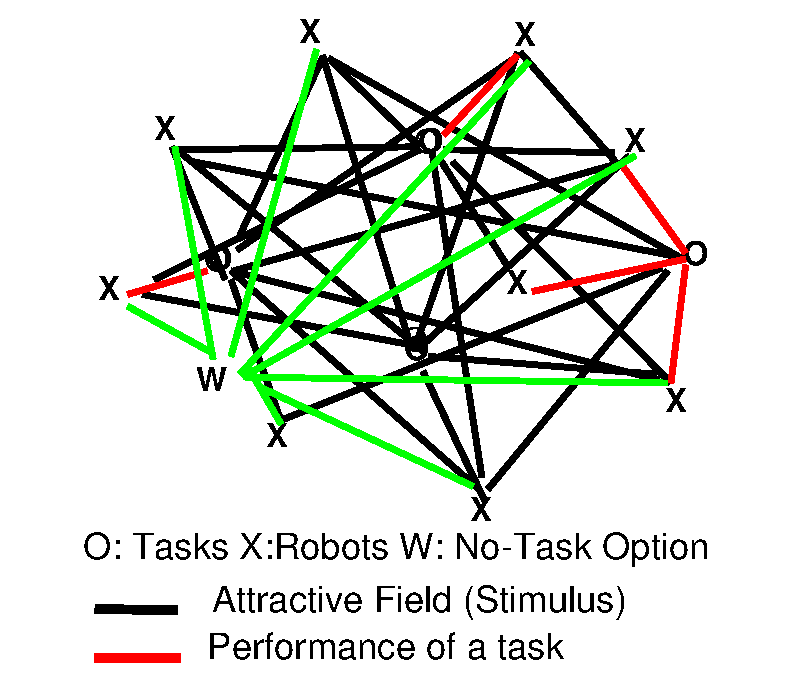
\includegraphics[height=4.5cm, angle=0]{../dia-files/AFM-Diag2.eps}
%figure caption is below the figur
\caption{\small Attractive Filed Model (AFM)}
\label{fig:afm} % Give a unique label
\end{minipage}
\hspace{0.5cm}
\begin{minipage}[t]{0.48\linewidth}
\centering
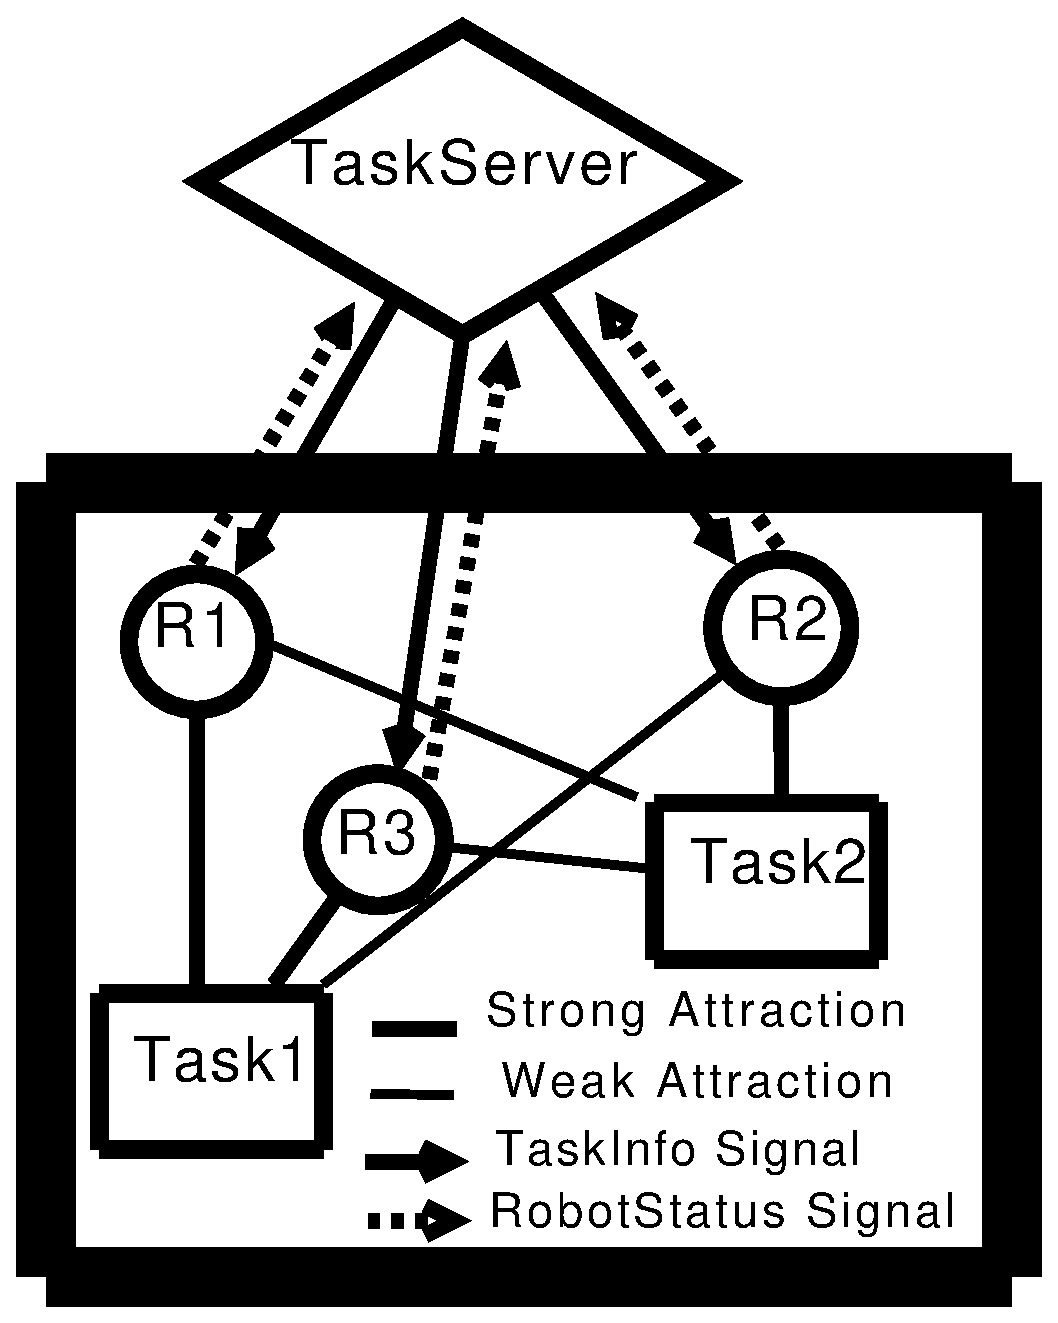
\includegraphics[height=4.5cm, angle=0]{../dia-files/CentralizedComm.eps}
\caption{\small A centralized communication scheme} % for implementing AFM}
\label{fig:ccm} % Give a unique label
\end{minipage}
\end{figure}
%%
Now let us interpret this model within the context of our MRS. Let us consider a manufacturing shop floor scenario where N number of mobile robots are required to attend to M number of shop tasks spread over a fixed area A.
Let these tasks be represented by a set of small rectangular boxes resembling to manufacturing machines.
Let $R_1$, $R_2$ … $R_n$ be the set of all robots and $J_1$, $J_2$ … $J_m$ be the set of all tasks.
Each task $j$ has an associated task-urgency $\phi_j$ that indicates its relative importance over time.
If a robot attends to a task $j$ in x$^{th}$ time-step, value of $\phi_j$ will decreases by a small amount $\delta_\phi$ in (x+1)$^{th}$ time-step.
On the other hand, if a task has not been served by any robot in x$^{th}$ time-step, $\phi_j$ will increase by another small amount in (x+1)$^{th}$ time-step.
In order to complete a shop task $J_1$, a robot $R_1$ needs to reach within a fixed boundary $D_{j1}$ of $J_1$.
If a robot completes a task $j$ we say that it learns about it and this will increase this robot's likelihood of selecting that task in next step.
We call this variable affinity of a robot to that task as its sensitization $k_j$.
If a robot does not do a task $j$ for some time, we say that it forgets about $j$ and $k_j$ has been decreased.\\
According AFM, all robots will establish attractive fields to all tasks due to the presence of a system-wide continuous flow of information.
The strength of these attractive fields called stimulus will vary according to the distances between robots and tasks, task-urgencies and corresponding sensitizations of robots. This is encoded in Eq. \ref{eqn1}.
%\addtolength{\abovedisplayskip}{-15mm}
\begin{small}
\begin{multicols}{2}
\begin{equation}
S_{j}^{i} = tanh\{\frac{k_{j}^{i}}{d_{ij}+\delta } \phi _{j}\}
\label{eqn1}
\end{equation}
\vspace*{0.25cm}
\begin{equation}
P_{j}^{i} = \frac{S_{j}^{i}}{\sum_{j}^{}S_{j}^{i}}
\label{eqn2}
\end{equation}
\end{multicols}
\end{small}
%\addtolength{\belowdisplayskip}{-1mm}
%\vspace{2mm}
Eq. \ref{eqn1} states that the stimuli of a robot $i$ to a particular task $j$, $S_{j}^{i}$ depends on $i$'s spatial distance to $j$, $d_{ij}$, level of sensitization to $j$, $k_{j}^{i}$, and perceived urgency of that task ($\phi _{j}$). We use a very small constant value $\delta$ to avoid division by zero when a robot has reached the task, Since $S_{j}^{i}$ is a probability function, it is chosen as a $tanh$ in order
to keep the values between 0 and 1. The probability of selecting each task has been determined by a probabilistic method outlined in Eq. \ref{eqn2}.
AFM suggests that concurrency of a self-regulatory system can be maintained by specifying at least two task options: doing a task and not doing a task. In robots, the latter can be be treated as random walking. So in any time-step a robot will choose from M+1 tasks. Let $T_a$ be the allocated time to accomplish a task. If $R_1$ can enter inside the task boundary within $T_a$ time it waits there until $T_a$ elapsed. Otherwise it will select a different task.\\
%%
\begin{figure}
\centering
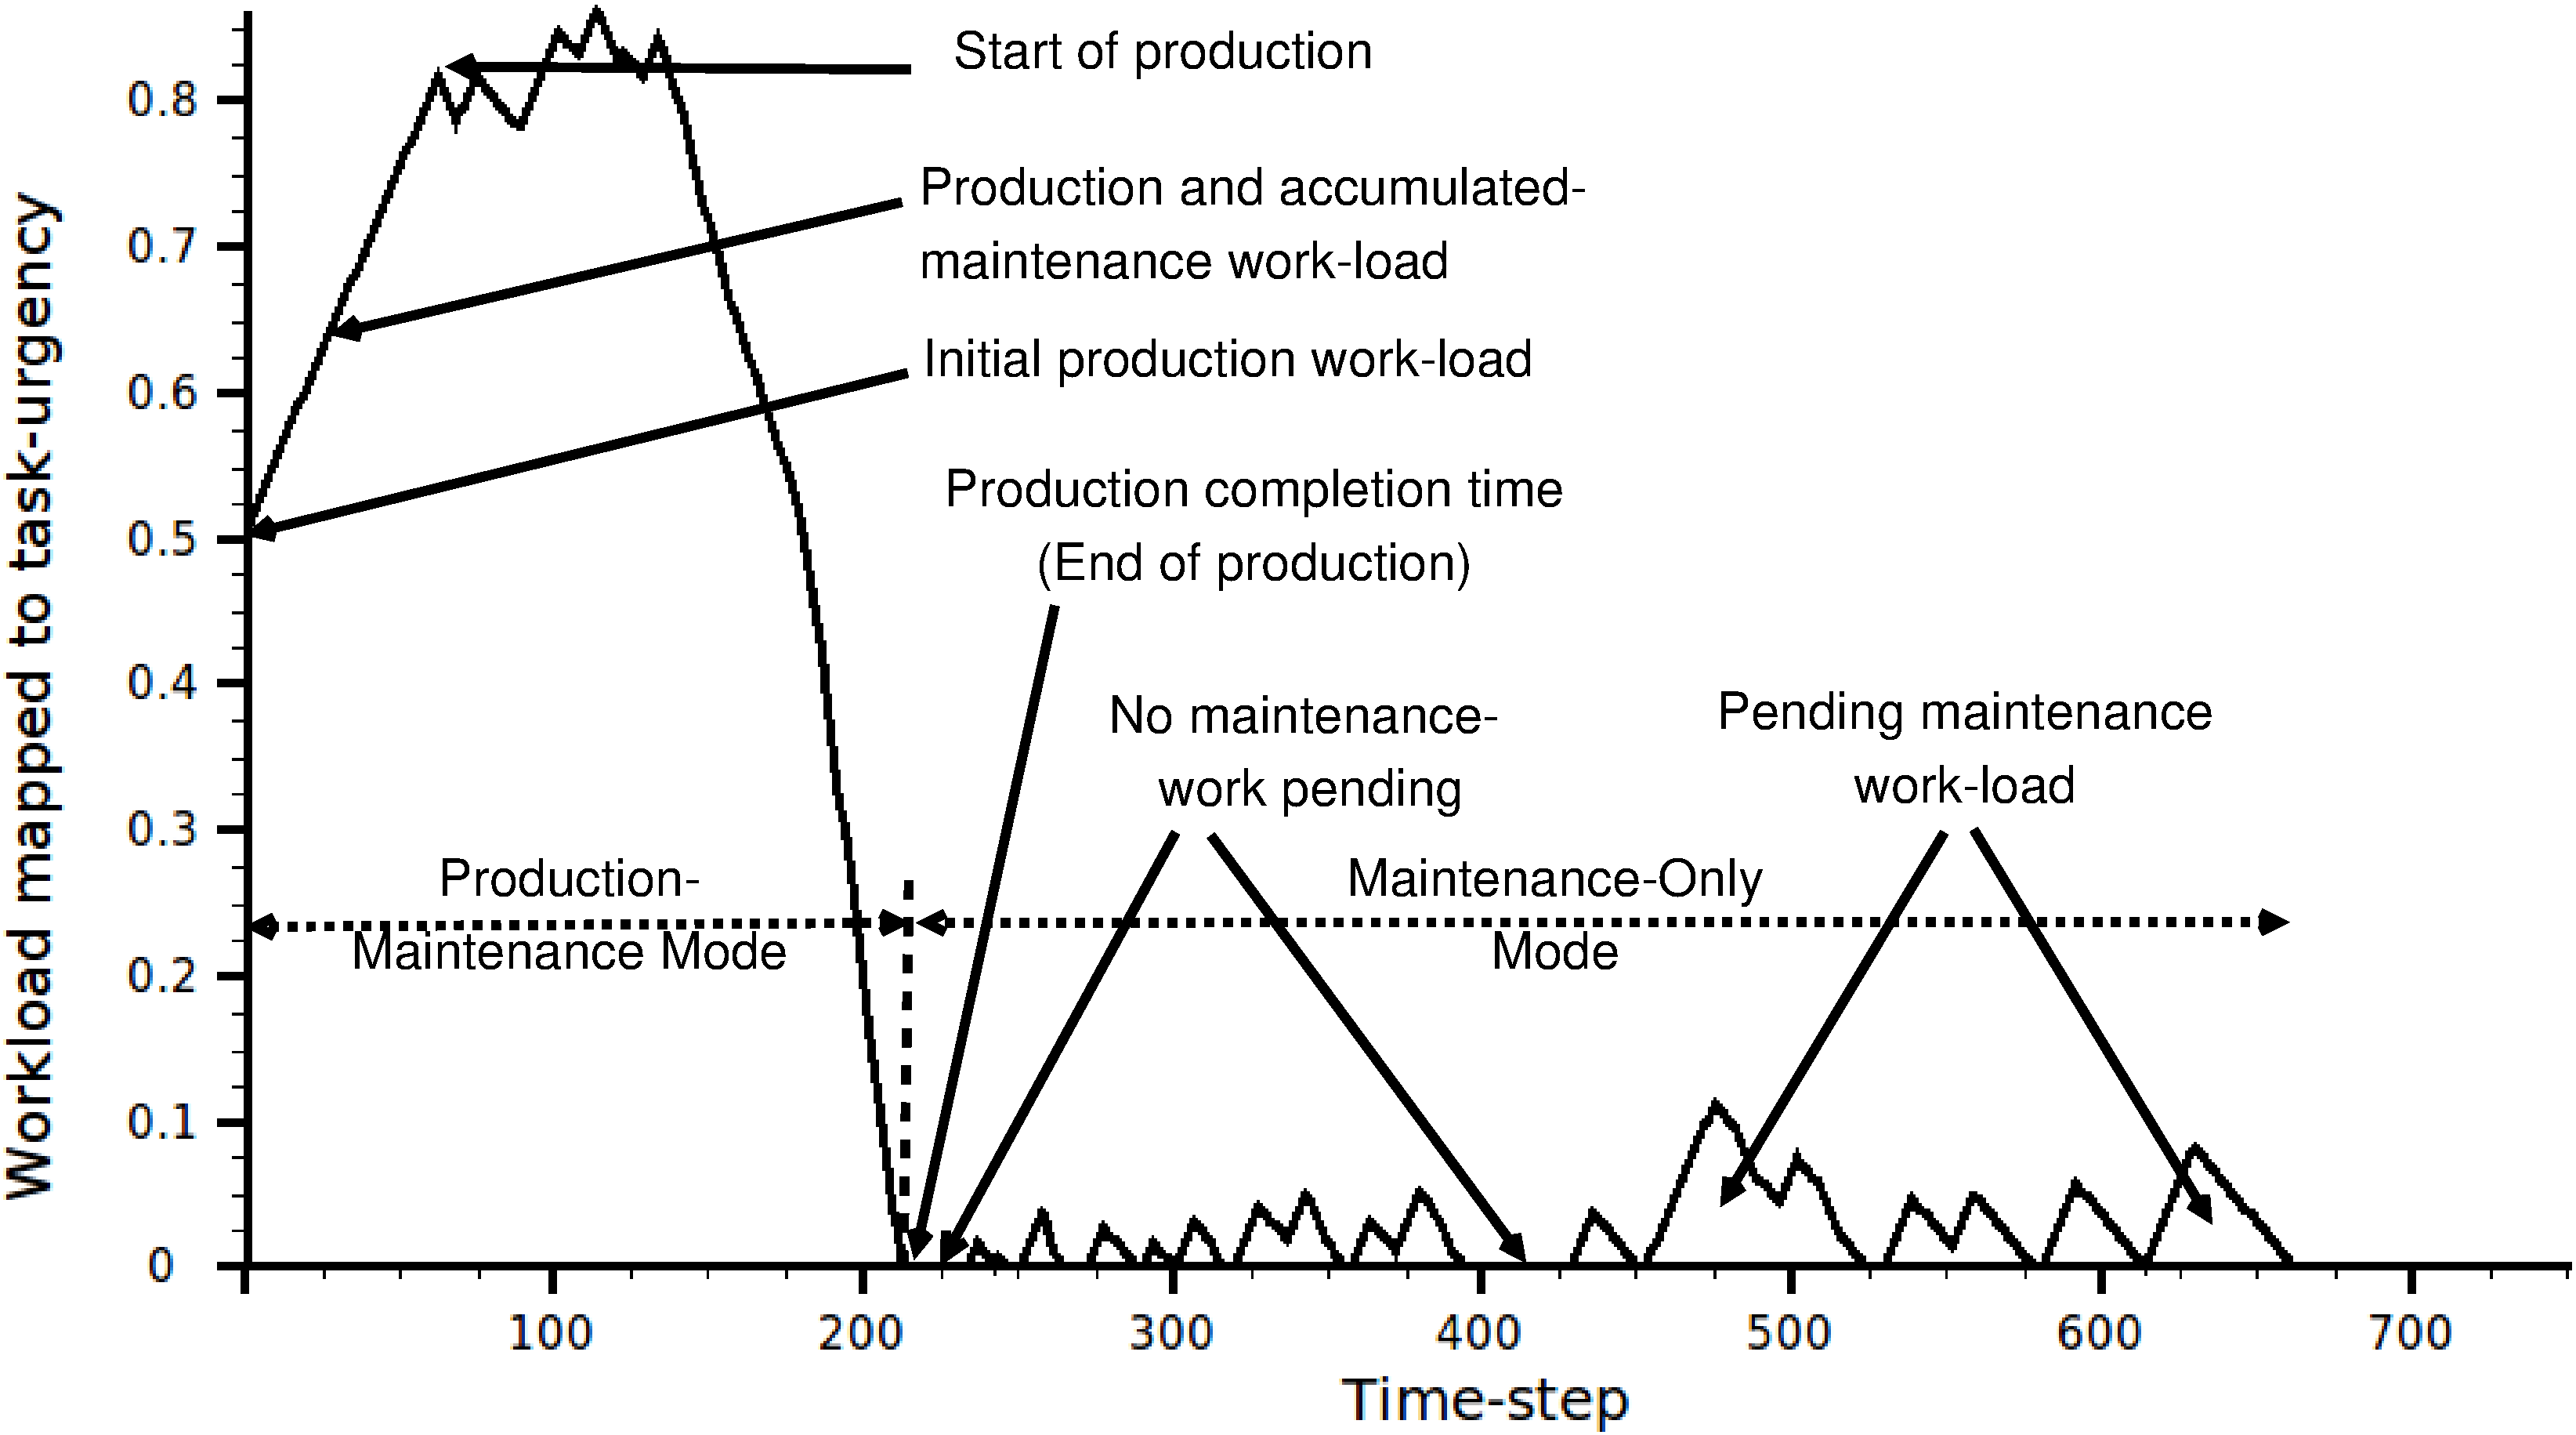
\includegraphics[width=12cm, angle=0]
{../dia-files/VSP.eps}
%figure caption is below the figure
\caption{\small Virtual Shop-floor production and maintenance cycle}
\label{fig:vsp}  % Give a unique label
\end{figure}
%%
In our manufacturing shop-floor scenario, each task represents a manufacturing machine. These machines are capable of producing goods from raw materials, but they also require constant maintenance works for stable operations. Let $W_{j}$ be a finite number of material parts that can be loaded into a machine $j$ in the beginning of its production process and in each time-step $\omega_{j}$ units of material parts can be processed  ($\omega_{j} \ll W_{j} $). So let $\Omega_{j}^{p}$ be the initial production workload of $j$ which is simply: $W_{j} / \omega_{j}$ unit. We assume that all machines are identical. In each time step, each machine always requires a minimum threshold number of robots, called hereafter as {\em minimum robots per machine ($\mu$)}, to meet its constant maintenance work-load, $\Omega_{j}^{m}$ unit. However, if $\mu$ or more robots are present in a machine for production purpose, we assume that, no extra robot is required to do its maintenance work separately. These robots, along with their production jobs, can do necessary maintenance works concurrently. For the sake of simplicity, in this paper we consider $\mu$ = 1.\\
Now let us fit the above production and maintenance work-loads and task performance of robots into a unit task-urgency scale. Let us divide our manufacturing operation into two subsequent stages: 1) {\em production and maintenance mode (PMM)}, and 2) {\em maintenance only mode (MOM)}. Initially a machine starts working in PMM and does production and maintenance works concurrently. When there is no production work left, it then enters into MOM. Fig. \ref{fig:vsp} illustrates this for a single machine.
Under both modes, let $\alpha_{j}$ be the amount of workload occurs in a unit time-step if no robot serves a task and it corresponds to a fixed task-urgency $\Delta \phi_{INC}$. On the other hand, let us assume that in each time-step, a robot, $i$, can decrease a constant workload $\beta_{i}$ by doing some maintenance work along with doing any available production work. This  corresponds to a negative task urgency: $- \Delta \phi_{DEC}$. 
So, at the beginning of production process, task-urgency, occurred in a machine due to its production work-loads, can be encoded by Eq. \ref{eqn:task-urgency-prod-init}.
\begin{equation}
%\small
\Phi_{j, INIT}^{PMM} = \Omega_{j}^{p} \times \Delta \phi_{INC} + \phi_{j}^{m0}
\label{eqn:task-urgency-prod-init}
\end{equation}
where $\phi_{j}^{m0}$ represents the task-urgency due to any initial maintenance work-load of $j$.
Now if no robot attends to serve a machine, each time-step a constant maintenance workload of $\alpha_{j}^{m}$ will be added to $j$ and that will increase its task-urgency by $\Delta \phi_{INC}$. So, if k time steps passes without any production work being done, task urgency at $k^{th}$ time-step will follow Eq. \ref{eqn:task-urgency-prod-case1}.
\begin{equation}
\Phi_{j, k}^{PMM} =\Phi_{j, INIT}^{PMM} + k \times \Delta \phi_{INC}
\label{eqn:task-urgency-prod-case1}
\end{equation}
However, if a robot attends to a machine and does some production works from it, there would be no extra maintenance work as we assumed that $\mu$ = 1. Rather, the task-urgency on this machine will decrease by $\Delta \phi_{DEC}$ amount. If $\nu_{k}$ robots work on a machine simultaneously at time-step $k$, this decrease will be: $\nu_{k} \times \Delta \phi_{DEC}$. So in such cases, task-urgency in $(k+1)^{th}$ time-step can be represented by:
\begin{equation}
\Phi_{j, k+1}^{PMM} = \Phi_{j, k}^{PMM} - \nu_{k} \times \Delta \phi_{DEC}
\label{eqn:task-urgency-prod-case2}
\end{equation}
At a particular machine $j$, once $\Phi_{j, k}^{PMM}$ reaches to zero, we can say that there is no more production work left and this time-step $k$ can give us the {\em production completion time} of $j$, $T_{j}^{PMM}$. Average production time-steps of a shop-floor with M machines can be calculated by the following simple equation.
\begin{equation}
T_{avg}^{PMM} = \frac{1}{M} \sum_{j=0}^{M} T_{j}^{PMM} 
\label{eqn:avg-pmm}
\end{equation}
$T_{avg}^{PMM}$ can be compared with the minimum number of time-steps necessary to finish production works, $T_{min}^{PMM}$. This can only happen in an ideal case where all robots work for production without any random walking or failure. We can get $T_{min}^{PMM}$ from the total amount of work load and maximum possible input from all robots. If there are M machines and N robots, each machine has $\Phi_{INIT}^{PMM}$ task-urgency, and each time-step robots can decrease N $times$ $\Delta \phi_{DEC}$ task-urgencies, then the theoretical $T_{min}^{PMM}$ can be found from the following Eq. \ref{eqn:min-pmm}.
%
\begin{equation}
T_{min}^{PMM} = \frac{M \times \Phi_{INIT}^{PMM}}{N \times \Delta \phi_{DEC}} 
\label{eqn:min-pmm}
\end{equation}
Thus using the above two terms we can define $\zeta_{avg}^{PMM}$, {\em average production completion delay} (APCD) as following:
\begin{equation}
\zeta_{avg}^{PMM} = \frac{T_{avg}^{PMM} - T_{min}^{PMM}}{T_{min}^{PMM}} 
\label{eqn:appd}
\end{equation}
%%
When a machine enters into MOM, only $\mu$ robots are required to do its maintenance works in each time step. So, in such cases, if no robot serves a machine, the growth of task-urgency will follow Eq. \ref{eqn:task-urgency-prod-case1}. However, if $\nu_{k}$ robots are serving this machine at a particular time-step $k^{th}$ , task-urgency at $(k+1)^{th}$ time-step can be represented by:
\begin{equation}
\Phi_{j, k+1}^{MOM} = \Phi_{j, k}^{MOM}- (\nu_{k} - \mu) \times \Delta \phi_{DEC}
\label{eqn:task-urgency-maint-case}
\end{equation}
By considering $\mu = 1$ Eq. \ref{eqn:task-urgency-maint-case} will reduces to Eq. \ref{eqn:task-urgency-prod-case2}. Here, $\Phi_{j, k+1}^{MOM}$ will correspond to the {\em pending maintenance work-load (PMW)} of a particular machine at a given time. This happens due to the random task switching of robots with a no-task option (random-walking). Interestingly PMW will indicate the robustness of this system since higher PMW value will indicate the delay in attending maintenance works by robots. We can find the average PMW (APMW) per time-step per machine, $\chi_{j}^{MOM}$ (Eq. \ref{eqn:sigle-pmw}) and averaging it for M machines of a shop-floor will give us average PMW per machine per time-step, $\chi_{avg}^{MOM}$ (Eq. \ref{eqn:avg-pmw}).
%\begin{multicols}{2}
%\small
\begin{equation}
\chi_{j}^{MOM}= \frac{1}{K} \sum_{k=1}^{K} \Phi_{j, k}^{MOM}
\label{eqn:sigle-pmw}
\end{equation}
%\vspace*{0.2cm}
\begin{equation}
\chi_{avg}^{MOM}= \frac{1}{M} \sum_{j=1}^{M} {\chi_{j}^{MOM}}
\label{eqn:avg-pmw}
\end{equation}
%\end{multicols}
%%
%%%%%%%%%%%%%%%%%%%%%%%%%%%%%%%%%%%%%%%%%%%%%%%%%%%%%%%%%%%%%%%%%%%%%%%%%%%%%%%%%%% 
\section{Implementation}
\label{sec:impl}
\begin{figure}
\centering
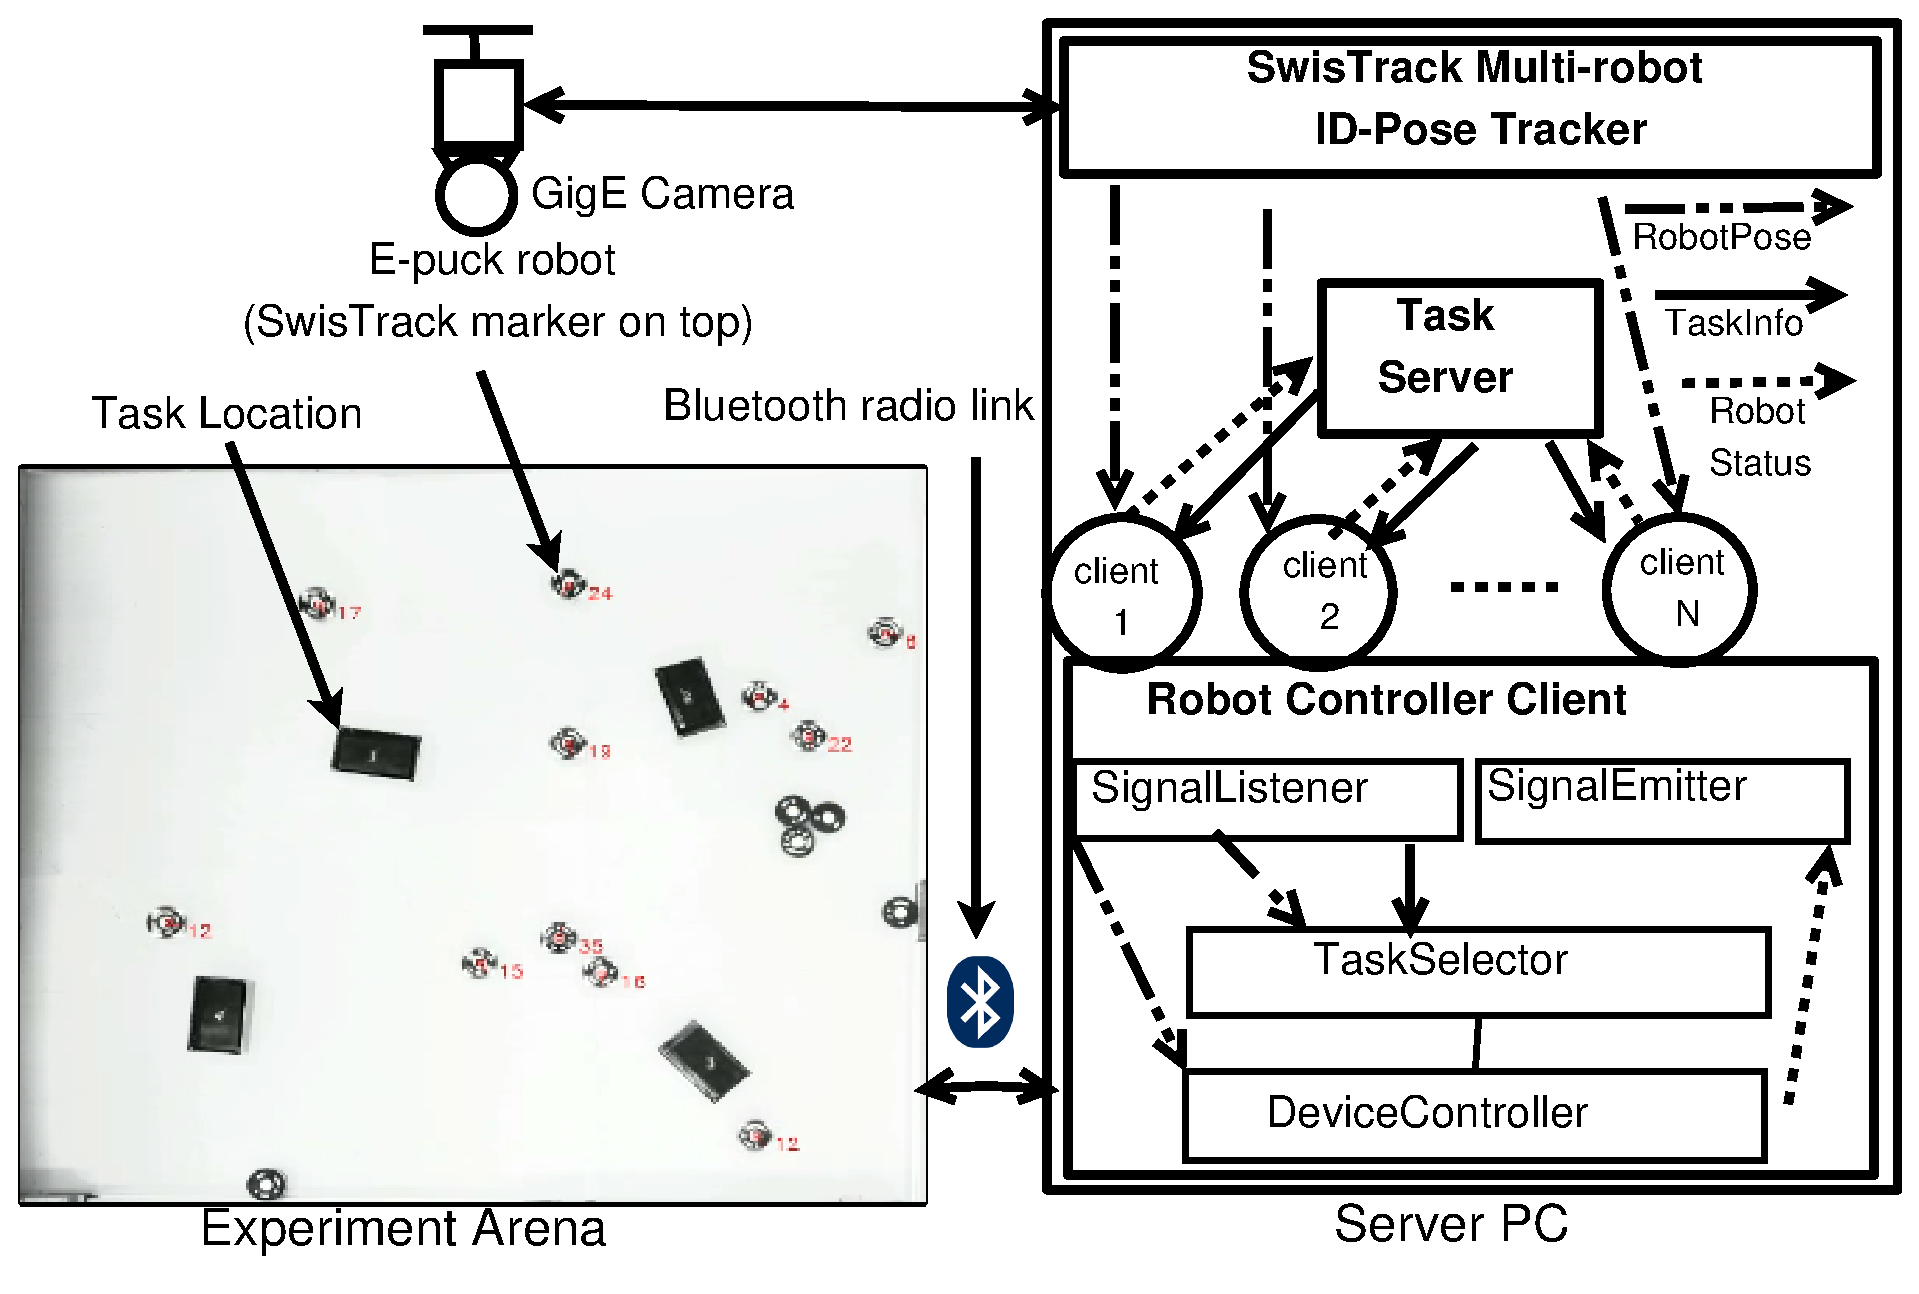
\includegraphics[height=5cm, angle=0]
{../dia-files/RIL-Expt-Setup1.eps}
%figure caption is below the figure
\caption{\small Hardware and software setup}
\label{fig:setup} % Give a unique label
\end{figure}
We have developed a system where up to 40 E-puck robots \footnote{www.e-puck.org} can operate together according to the generic rules of the AFM. As shown in Fig. \ref{fig:setup}, our software system consists of a multi-robot tracking system, a centralized task server and robot controller clients. Here at first we have presented the design of our communication system. Then we have discussed about our specific implementation. 
%%%
\subsection{Design of our communication system}
In order to establish a system-wide continuous flow of information, we need to implement a suitable communication system for our robots. Here we have presented a centralized communication system for our manufacturing shop-floor scenario.
%% 
As shown in Fig. \ref{fig:ccm}, in this model there exists a centralized \textit{
TaskServer} that is responsible for disseminating task information to robots. The contents of task information can be physical locations of tasks, their urgencies and so on. TaskServer delivers this information by emitting \textit{TaskInfo} signals periodically. The method of signal emission depends on a particular communication technology. For example, in a wireless network it can be a message broadcast.
Task-Server has another interface for catching feedback signals from robots. The \textit{RobotStatus} signal can be used to inform TaskServer about a robot's current task id, its device status and so on. TaskServer uses this information to update relevant part of task information such as, task-urgency. This up-to-date information is sent in next TaskInfo signal.\\
In Fig. \ref{fig:ccm} an initial configuration of this model has been presented. Upon receiving an initial TaskInfo signal robot $R_1$ has shown strong attraction towards $Task1$ and robot $R_3$ has shown strong attraction toward $Task2$. This can be inferred from Eq. \ref{eqn1} that says if the initial task urgencies and sensitizations for all tasks are same, a robot will strongly be attracted towards a task that is relatively closer to it.
\subsection{Our current implementation}
The major components of our implementation are a multi-robot tracking system, robot controller clients and a centralized task-server. In order to track all robots real-time we have used SwisTrack \cite{SwisTrack}, a state of the art open-source, multi-agent tracking system, with a16-megapixel overhead GigE camera. This set-up gives us the position, heading and id of each of the robots at a frequency of 1. The interaction of the hardware and software of our system is illustrated in Fig. \ref{fig:setup}. \\
For inter-process communication (IPC), we have used D-Bus technology \footnote{http://dbus.freedesktop.org/doc/dbus-specification.html}. We have developed an IPC component for SwisTrack (hereafter called as \textit{SwisTrack D-Bus Server}) that can broadcast id and pose of all robots in real-time over our server's D-Bus interface.\\
Apart from SwisTrack, we have implemented two major software modules: {\em TaskServer} and {\em Robot Controller Client (RCC)}. They are developed in Python with its state of the art \textit{Multiprocessing} \footnote{http://docs.python.org/library/multiprocessing.html} module. This python module simplifies our need to manage data sharing and synchronization among different sub-processes. As shown in Fig. \ref{fig:setup}, RCC consists of four sub-processes. {\em SignalListener} and {\em SignalEmitter}, interface with SwisTrack D-Bus Server and TaskServer respectively. {\em TaskSelector} implements AFM guidelines for task selection . {\em DeviceController} moves a robot to a target task. Bluetooth radio link is used as a communication medium between a RCC and a corresponding E-puck robot. 
%%%%%%%%%%%%%%%%%%%%%%%%%%%%%%%%%%%%%%%%%%%%%%%%%%%%%%%%%%%%%%%%%%%%%%%%%%%%
\section{Experiment Design}
\label{sec:expt-design}
In this section, we have described the design of parameters and observables of our experiments.
These experiments are designed to validate AFM by testing the occurrence of convergent MRTA. Our experimental setup can be found in section~\ref{sec:impl}. The details of convergence is presented in section~\ref{sec:results}.
%
\begin{table}
\caption{Experimental parameters}
\label{table:params}
\begin{center}
\begin{tabular}{|l||c|}
\hline Parameter & Value\\
\hline Total number of robots ($N$) & 16\\
\hline Total number of tasks ($M$) & 4\\
\hline Experiment area ($A$) & 4 $m^2$\\
\hline Initial production work-load/machine ($\Omega_{j}^{p}$) & 100 unit\\
\hline Task urgency increase rate ($\Delta\phi_{INC}$) & 0.005\\
\hline Task urgency decrease rate ($\Delta\phi_{DEC}$) & 0.0025\\
\hline Initial sensitization ($K_{INIT}$) & 0.1\\
\hline Sensitization increase rate ($\Delta k_{INC}$) & 0.03\\
\hline Sensitization decrease rate ($\Delta k_{DEC}$) & 0.01\\
%\hline A very small distance ($\delta$)& 0.000001\\
\hline Task info update interval ($\Delta TS_{u}$) & 5s\\
%\hline Task info signal emission interval ($ \Delta TS_{e}$)& 2.5s\\
\hline Robot's task time-out interval ($\Delta RT_{to} $)& 10s\\
\hline
\end{tabular}
\end{center}
\end{table}
% 
\subsection{Parameters}
Table \ref{table:params} lists a set of essential parameters of our experiments. We intend to have a setup that is relatively complex, i.e., a high number of robots and tasks in a large area, but with a high probability of convergence. The diameter of the marker of our E-puck robot is 0.08m. So, if we put 4 robots in an area of one square meter, this will give us a robot-occupied-space to free-space ratio of about 1:49 per square meter. We have found that this ratio reasonable in order to allow the robots to move at a speed of 7.5 cm/sec (half of their maximum possible speed) without much interference to each other. We have fixed the number of task to 4. They also have an additional option for random walking. So the total number of tasks becomes 5. This gives our robots a relatively high number of tasks to work on. \\
%When many Bluetooth devices talk to a single Bluetooth adapter, communication delays become very frequent due to the fact that each device gets a guaranteed turn to communicate \cite{Bluetooth}.
% In order to provide robots with a higher degree of access to Bluetooth communication links, we intend to dedicate one Bluetooth adapter for each robot. This would ensure that communication delays do not hamper a robot's task performance. However too many Bluetooth adapters caused our server PC to crash frequently. We have found a stable server configuration with 8 Bluetooth adapters, i.e., one Bluetooth adapter is used to communicate with two robots. This limits us to set the total number of robots to 16. Also we found that after about 35-40 minutes from the start of our experiments some of robots fail to get the access to their designated Bluetooth adapters. So we limit the length of our experiments to 40 minutes. We expect that this limitation would be removed by distributing Bluetooth adapters among multiple server PCs.\\ 
The initial values of task urgencies can be set to any value as long as they are same for all tasks. We choose a limit of 0 and 1, where 0 means no urgency and 1 means maximum urgency. Same applies to sensitisation as well, where 0 means no sensitisation and 1 means maximum sensitisation. This also implies that if sensitization is 0, task has been forgotten completely. On the other hand, if sensitization is 1, the task has been learnt completely. We choose a default sensitization value of 0.1 
for all tasks. The following relationships are maintained for selecting task-urgency and sensitization parameters.
\begin{small}
\begin{equation}
\Delta\phi_{INC} =  \frac{\Delta\phi_{DEC} \times N}{2 \times M}
\label{eqn:task-urgency}
\end{equation}
%
\begin{equation}
\Delta k_{DEC} = \frac{\Delta k_{INC}} {M - 1} 
\label{eqn:sensitization}
\end{equation}
\end{small}
%
Eq. \ref{eqn:task-urgency} establishes the fact that task urgency will increase at a higher rate than that of its decrease. As we do not like to keep a task left unattended for a long time we choose a higher rate of increase of task urgency. This difference is set on the basis of our assumption that at least half of the expected number of robots (ratio of number of robots to tasks) would be available to work on a task. So they would produce similar types of increase and decrease behaviours in task urgencies.\\
Eq. \ref{eqn:sensitization} suggests that the learning will happen much faster than the forgetting. The difference in these two rates is based on the fact that faster leaning gives a robot more chances to stick on to it. The exact ratio of learning and forgetting is related here by the fact that if a robot works on a task it learns about it and forgets about the rest. 
\subsection{Observables}
We have defined a set of observables to benchmark our implementation. The first two observables, the changes in task-urgencies and the changes in robot sensitizations, give us an external and an internal view of our system with respect to AFM respectively. Our third observable is to find changes in robot motions. This is completely objective measurement of our system.% Our final measurement is the communication load which is specific to this particular implementation. They are briefly explained here.\\
%\textbf{Changes in task-urgencies ($\Delta \Phi$): }
%In our experiments, urgency of each task in each step has been logged. %From the above design of task urgency, we can see that if a task is not served by any robot for 100 consecutive steps (500s), urgency of that task will reach from 0.5 to its maximum value 1.0. On the other hand, if a task is served by only one robot for 200 consecutive steps (1000s) urgency of that task will be 0. But in real experiment, it is more likely that more than one robot will serve a task. So urgency of a task will decrease $\Delta\phi_{DEC}$ times number of working robots on that task (based on AFM guidelines \cite{Elsa}).\\ %The overall changes in task urgencies will show the convergence behaviour of our system. A stable convergence will most likely map to a stable division of labour of the system.\\
%\textbf{Changes in robot sensitizations ($\Delta K$): }
%According AFM, as robots will do tasks they will specialize on each task by increasing or decreasing sensitizations (learning and forgetting). From our above design, we can see that if a robot starts doing a task with an initial sensitization of 0.1 and it repeatedly does it for 30 consecutive steps, we will be able to say that it has learnt it completely. On the other hand, with an initial sensitization of 0.1 if a robot does not do a task for 10 consecutive steps we will be able to say that it has forgotten that task completely.\\
%\textbf{Changes in robot motions ($\Delta U$): }
%As we might guess that initially the task urgencies will be relatively higher for all tasks so robots will need to do a lot of movements by switching from one tasks to another. But as the system convergences overall robot motions will be decreased. In order to observe this phenomenon we log the pose of robots in each time they receive pose signals.
%\textbf{D-Bus Signals emitted by Task server ($S_f$):} 
%In order to measure the communication load on our system and to benchmark Task server's D-Bus signalling performance we are also interested to log TaskInfo D-Bus signals. Since the emission of signals happens in a fixed time interval it is more likely that the overall communication load on the system will remain constant over time.
%
%%%%%%%%%%%%%%%%%%%%%%%%%%%%%%%%%%%%%%%%%%%%%%%%%%%%%%%%%%%
% 
\section{Results and Discussions}
\label{sec:results}
%%
In this section we have presented our experimental results. We ran those experiments for about 40 minutes and averaged them from three iterations.
Fig. \ref{fig:raw-urgencies} shows the dynamic changes in task urgencies. Here we find that at about $100^{th}$ step all urgencies has stabilized near 0. The rise and fall of task urgencies show that our system is capable of providing a robust DoL. 
In order to describe our system's dynamic behaviour holistically we analyse the changes in task urgencies over time. Let $ \phi_{j, q}$ be the urgency of a task $j$ at $q^{th}$ step. In $(q+1)^{th}$ step, we can find the change of urgency of task $j$ :\\
\begin{equation} 
\small
\delta \phi_{j, q+1} = ( \phi_{j, q+1} - \phi_{j, q}) 
\end{equation}
So we can calculate the sum of changes in urgencies of all tasks at $(q+1)^{th}$ step:
\begin{equation} 
\small
\Delta \Phi_{j, q+1} = \sum_{j=1}^{M} \delta \phi_{j, q+1} 
\label{eqn:Delta-Phi}
\end{equation}
Fig. \ref{fig:urgency-convergence} plots this sum of changes of task urgencies by a dashed line. If we consider the absolute change over a window $w$ of time in the following equation we can describe the overall changes of our systems in both positive and negative directions.
%
\begin{equation}
\small
\Delta \Phi_{jw, q+1} = \sum_{j=0}^{w-1} \left | \Delta \Phi_{q+j} \right |
\end{equation}
%
In order to find convergence in DoL we have calculated the sum of absolute changes in task urgencies over a window of 2 consecutive steps (100s). This is plotted in solid line in Fig. \ref{fig:urgency-convergence}. Note that we scale down the time steps of this plot by aggregating the values of 10 consecutive steps (50s) of Fig. \ref{fig:raw-urgencies} into a single step value.
From Fig. \ref{fig:raw-urgencies} we can see that initially the sum of changes of task urgencies are towards negative direction. This implies that tasks are being served by a high number of robots.
%When the task urgencies stabilize near zero the fluctuations in urgencies become minimum. Since robots chose tasks stochastically, there will always be a small changes in task urgencies. %A potential convergence point is shown in Fig. \ref{fig:urgency-convergence} by considering the persistence existence of the value of $\Delta \Phi_{jw, q+1}$ below a threshold 0.1. This convergence happens near step 23 or after 1150s from the beginning of our experiments. This implies that from this point of time and onwards, changes of our system's behaviour remains under a small threshold value.\\
%
Similar to Eq. \ref{eqn:Delta-Phi}, we can calculate the absolute sum of changes in sensitizations by all robots in the following equation.
% 
\begin{equation}
\small 
\Delta K_{j, q+1} = \sum_{j=1}^{M} \left | \Delta k_{j, q+1} \right |
\label{eqn:Delta-K}
\end{equation}
This values of $\Delta K$ are plotted in Fig. \ref{fig:sensitization-stat}. It shows that the overall rate of learning and forgetting decrease over time. It is a consequence of the gradually increased task specialization of robots.
%%
We have aggregated the changes in translation motion of all robots over time. Let $u_{i,q}$ and $u_{i,q+1}$ be the translations of a robot $i$ in two consecutive steps. If the difference between these two translations be $\delta u_{i}$, we can find the sum of changes of translations of all robots in $(q+1)^{th}$ step using the following equation.
\begin{equation}
\small 
\Delta U_{q+1} = \sum_{i=1}^{N} \delta u_{i, q+1} 
\label{eqn:Delta-Tr}
\end{equation}
This is plotted in Fig. \ref{fig:translation-stat}. In this plot we can see that robot translations also vary over varying task requirements of tasks.\\ %But it fails to show a consistence behaviour like previous plots.\\
As an example of task specialization of a robot we plotted sensitization of Robot9 in Fig. \ref{fig:single-robot-sensitizations}. It shows that this robot has specialized in Task1. The continuous learning happens from step 12 to step 42 where it has learned this task completely and forgot rest of the tasks. This behaviour is found common in all robots with varying level of sensitizations. Hence we get the linear decrease of $\Delta K$ in Fig. \ref{fig:sensitization-stat}. However, the changes in motion of this robot plotted in Fig. \ref{fig:single-robot-translation} is not stable due to the fact that robots frequently avoid dynamic obstacles and select random-walking.
%%
\begin{figure}
\begin{minipage}[t]{0.48\linewidth}
\centering
\includegraphics[height=4.5cm, angle=0]
{images/PlotUrgencyLog-2010May10-115549.eps}
%figure caption is below the figure
\caption{\small Task urgencies observed at TaskServer}
\label{fig:raw-urgencies} % Give a unique label
\end{minipage}
\hspace{0.5cm}
\begin{minipage}[t]{0.48\linewidth}
\centering
\includegraphics[height=4.5cm, angle=0]{images/TaskUrgencyStat.eps}
\caption{\small Shop-floor workload change history measured in terms of task urgencies}
\label{fig:urgency-convergence} % Give a unique label
\end{minipage}
\end{figure}
%%
%%% Sensitization and Translation %%%
\begin{figure}
\begin{minipage}[t]{0.48\linewidth}
\centering
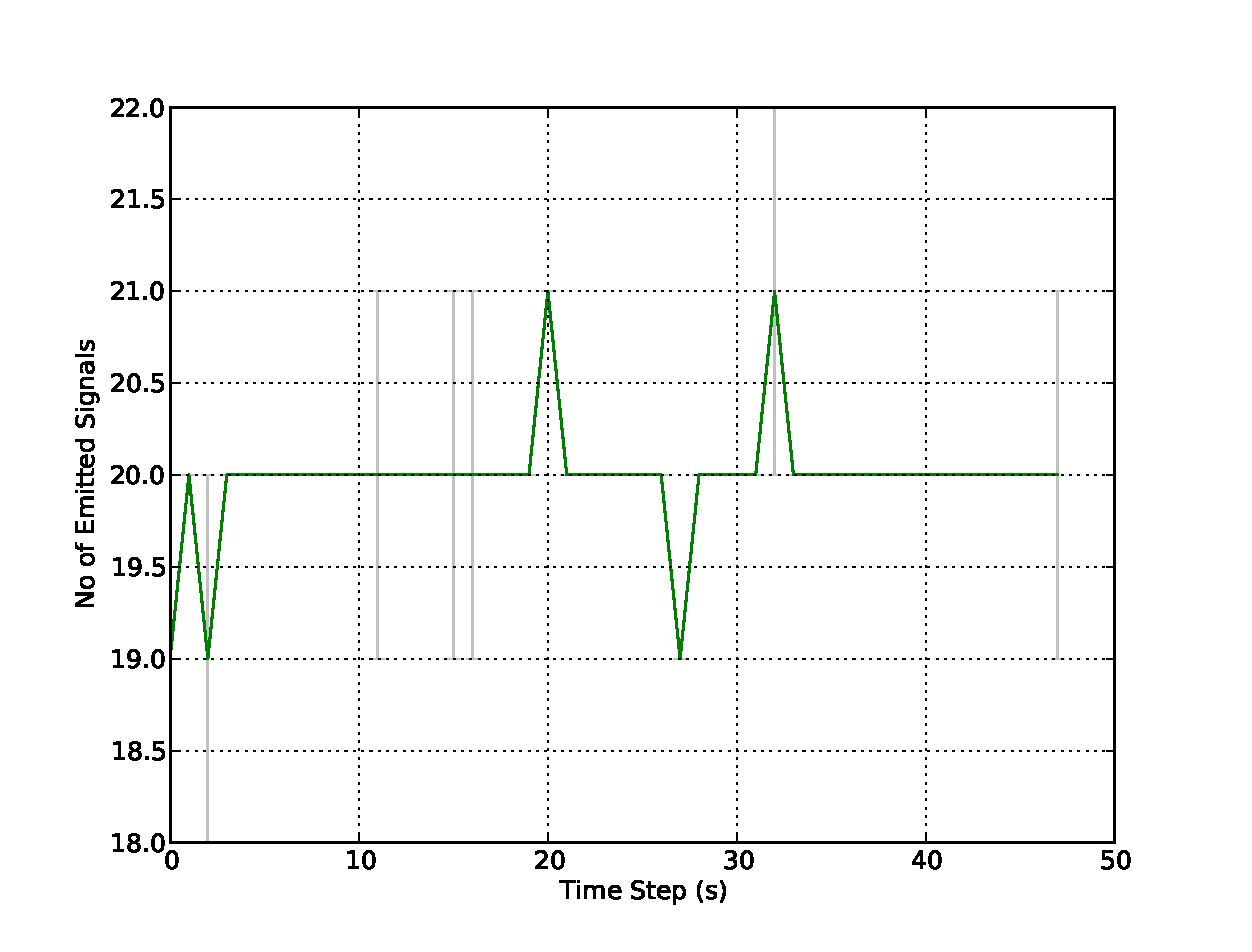
\includegraphics[height=4.5cm, angle=0]
{images/global/Global-SignalingFreqStat.eps}
%figure caption is below the figure
\caption{\small Task server's frequency of task information signalling}
\label{fig:signal-frequency-stat}
%
\end{minipage}
\hspace{0.5cm}
\begin{minipage}[t]{0.48\linewidth}
\centering
\includegraphics[height=4.5cm, angle=0]{images/WorkerRatio.eps}
\caption{\small Self-organized allocation of working robots }
\label{fig:translation-stat} % Give a unique label
\end{minipage}
\end{figure}
%%
%%% Communication load %%%
%\begin{figure}
%\begin{minipage}[t]{0.5\linewidth}
%\centering
%\includegraphics[height=4.5cm, angle=0]
%{images/global/Global-SignalingFreqStat.eps}
%figure caption is below the figure
%\caption{\small Task server's frequency of task information signalling}
%\label{fig:signal-frequency-stat} % Give a unique label
%\end{minipage}
%\end{figure}
%Fig. \ref{fig:signal-frequency-stat} presents the frequency of signalling task information by TaskServer. Since the duration of each time step is 50s long and TaskServer emits signal in every 2.5s, there should be 20 signals in each step. The insignificant variation in frequency shows us the stable behaviour of D-Bus daemon over time.
\begin{figure}
\begin{minipage}[t]{0.48\linewidth}
\centering
\includegraphics[height=4.5cm, angle=0]{images/TaskSpecialization-task3-10may-1.eps}
\caption{\small Task specialization on Task3}
\label{fig:single-robot-sensitizations} % Give a unique label
\end{minipage} 
%%%
\hspace{0.5cm}
\begin{minipage}[t]{0.48\linewidth}
\centering
%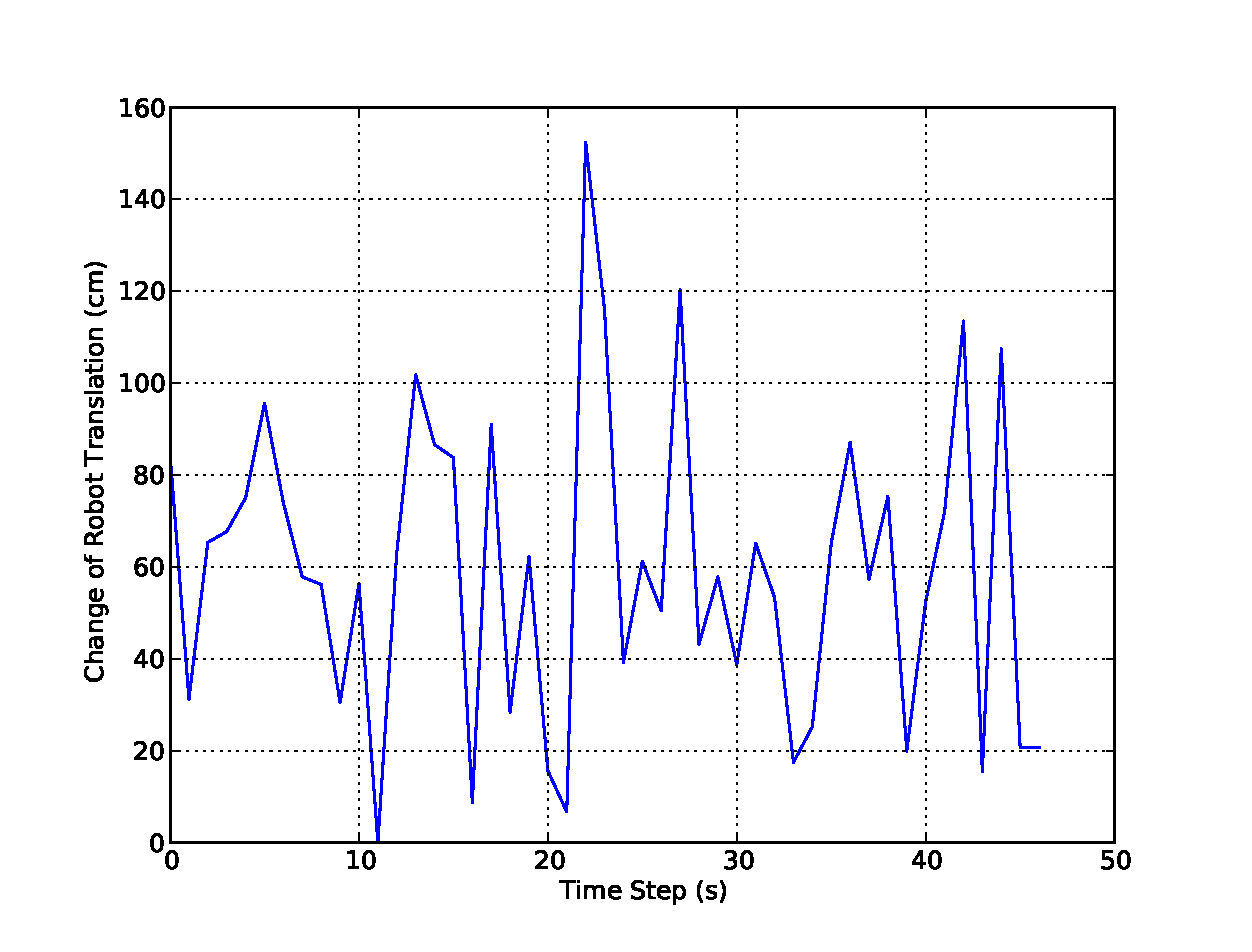
\includegraphics[height=4.5cm, angle=0]{images/global/DeltaRobot9-PoseAtTS-2010Feb18-121037.eps}
%\caption{\small Changes in translation of Robot9}
%\label{fig:single-robot-translation} % Give a unique label
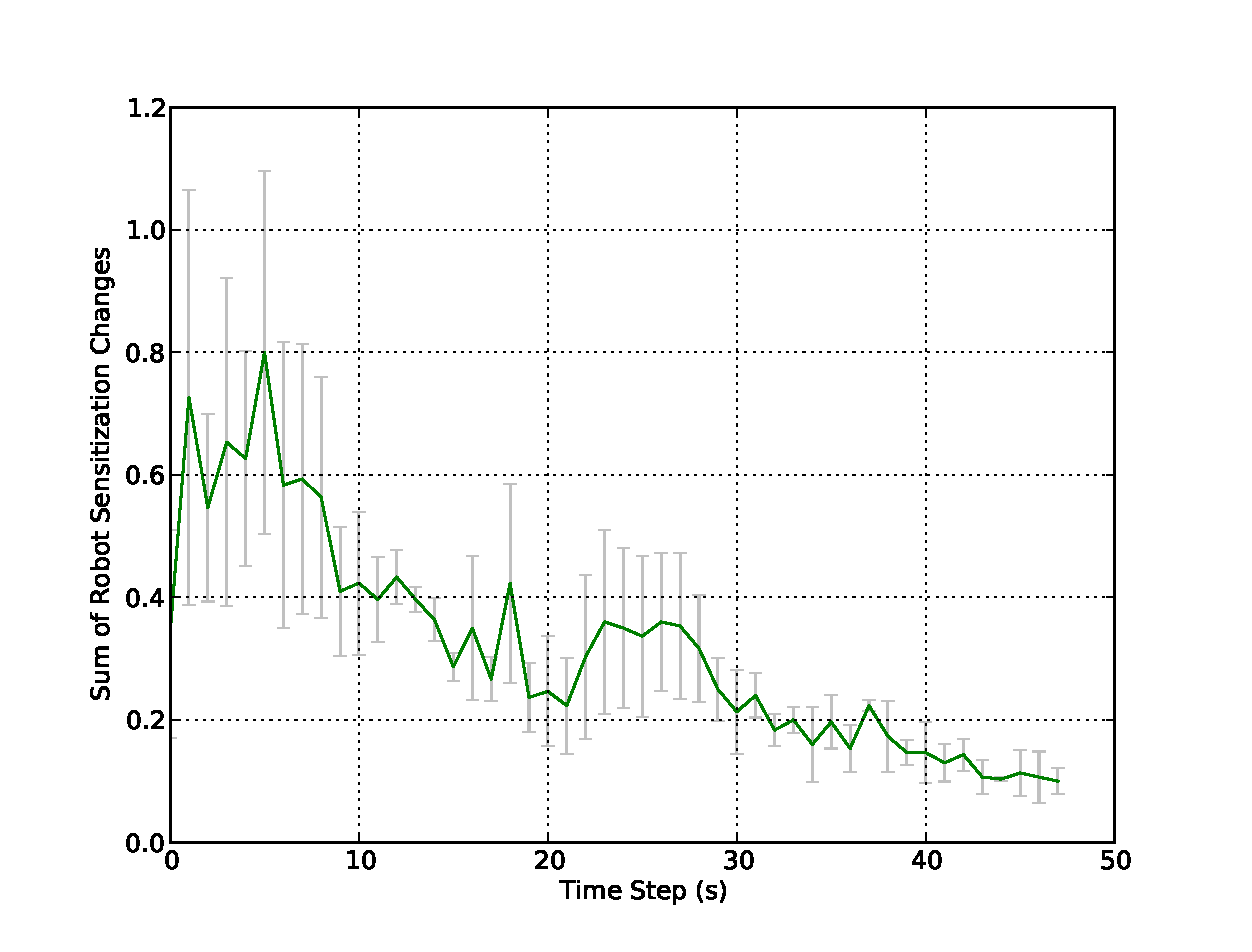
\includegraphics[height=4.5cm, angle=0]
{images/global/RobotSensitizationStat-Total-50steps.eps}
\caption{\small Changes in sensitizations of all robots}
\label{fig:sensitization-stat} % Give a unique label
\end{minipage}
\end{figure}
%%%%%%%%%%%%%%%%%%%%%%%%%%%%%%%%%%%%%%%%%%%%%%%%%%%%%%%%%%%%%%%%
\section{Conclusion and Future works}
\label{sec:conc}
In this paper we have validated an inter-disciplinary generic model of self-regulated division of labour by incorporating it in our multi-robot system (MRS). A centralized communication system has been instantiated to realize this model. We have evaluated various aspects of this model, such as ability to meet dynamic task demands, individual task specializations, communication loads and flexibility in concurrent task completions. A set of metrics has been proposed to observe the convergence of MRTA in this system. From our experimental results, we have found that AFM can meet the requirements of dynamic MRTA by the virtue of its self-regulatory behaviours. Our centralised communication system broadcasts information to all the robots from a central server. This has the advantage of minimising the communication load and the disadvantage of a single point of failure. In the future, we will explore local peer-to-peer communication models in a MRS having about 40 E-puck robots.
%%
\bigskip
\subsubsection*{Acknowledgements. } 
This research has been funded by the Engineering and Physical Sciences Research Council (EPSRC), UK, grant reference EP/E061915/1.
%\begin{acknowledgements}
%If you'd like to thank anyone, place your comments here
%and remove the percent signs.
%\end{acknowledgements}
% BibTeX users please use one of
%\bibliographystyle{spbasic} % basic style, author-year citations
%\bibliographystyle{spmpsci} % mathematics and physical sciences
%\bibliographystyle{spphys} % APS-like style for physics
%\bibdata{bib-intro}
%\bibliography{bib-intro} % name your BibTeX data base
% Non-BibTeX users please use
\begin{thebibliography}{}
% and use \bibitem to create references. Consult the Instructions
% for authors for reference list style.
%\bibitem{Camazine+2001}
%Camazine, S., Franks, N., Sneyd, J., Bonabeau, E., Deneubourg, J. and Theraulaz, G.: Self-organization in biological systems.
%Princeton University Press, Princeton, N.J (2001)
\bibitem{Bonabeau+1999}
Bonabeau, E., Dorigo, M. and Theraulaz, G.:
Swarm intelligence: from natural to artificial systems.
Oxford University Press (1999)
\bibitem{Gerkey+2004}
Gerkey, B. P. and Mataric M. J.:
A Formal Analysis and Taxonomy of Task Allocation in Multi-Robot Systems.
The International Journal of Robotics Research, 23 (2004)
\bibitem{Parker2008}
Parker, L. E.:
Distributed Intelligence: Overview of the Field and its Application in Multi-Robot Systems.
Journal of Physical Agents, 2, 5-14 (2008)
\bibitem{Lerman+2006}
Lerman, K., Jones, C., Galstyan, A. and Mataric, M. J.:
Analysis of Dynamic Task Allocation in Multi-Robot Systems. 
The International Journal of Robotics Research, 25, 225 (2006)
\bibitem{Shen+2001}
Shen, W., Hao, Q., Yoon, H. and Norrie, D.:
Applications of agent-based systems in intelligent manufacturing: An updated review. Advanced Engineering Informatics, 20, 415-431, Elsevier (2006)
\bibitem{Dias+2006}
Dias, M. B., Zlot, R. M., Kalra, N. and Stentz, A.:
Market-based multirobot coordination: A survey and analysis. 
Proceedings of the IEEE, 94, 1257-1270, IEEE (2006)
\bibitem{Liu+2007} 
Liu, W., Winfield, A. F. T., Sa, J., Chen, J. and Dou, L.:
Towards Energy Optimization: Emergent Task Allocation in a Swarm of Foraging Robots. Adaptive Behavior, 94, 1257-1270 (2007)
\bibitem{Sayer+1992}
Sayer, A. and Walker, R.: 
The new social economy : reworking the division of labor.
Blackwell (1992)
%\bibitem{Beer1981}
%Beer, S.: 
%Brain of the firm.
%J. Wiley New York (1981)
\bibitem{Kogut2000}
Kogut, B.: 
The network as knowledge: generative rules and the emergence of structure. 
Strategic Management Journal, 21, 405-425 (2000)
\bibitem{Swarm}
% Format for Journal Reference
Sahin E. and Winfield A.: 
Special issue on swarm robotics.
Swarm Intelligence, 2, 69-72 (2008)
% Format for books
\bibitem{Elsa}
Arcaute, E.; Christensen, K.; Sendova-Franks, A.; Dahl, T.; Espinosa, A. and Jensen, H. J. : 
Division of labour in ant colonies in terms of attractive fields. 
Ecological Complexity, Elsevier (2008)
% etc
\bibitem{SwisTrack}
Lochmatter T., Roduit P., Cianci C., Correll N., Jacot J., and Martinoli A.: 
SwisTrack - A Flexible Open Source Tracking Software for Multi-Agent Systems. 
In Proceedings of the IEEE/RSJ 2008 International Conference on Intelligent Robots and Systems (IROS 2008), 4004-4010, IEEE (2008)
%\bibitem{Epuck}
%Mondada, F., Bonani, M., Raemy, X., Pugh, J., Cianci, C., Klaptocz, A., Magnenat, S., %Zufferey, J.-C., Floreano, D. and Martinoli, A.:
%The e-puck, a Robot Designed for Education in Engineering. 
%Proceedings of the 9th Conference on Autonomous Robot Systems and Competitions, 1(1) %59-65 (2009)
%\bibitem{Bluetooth}
%Huang, A.S. and Rudolph, L.:
%Bluetooth essentials for programmers.
%Cambridge University Press (2007).
\end{thebibliography}
%
\end{document}
